\documentclass[/home/hernan/Documentos/Apuntes_mecanica_teorica/main.tex]{subfiles}
\graphicspath{{\subfix{images/}}}

\begin{document}
    \section{Sistemas de partículas}
    \label{sec: sisparticulas}

    Para trabajar con sistemas de partículas es necesario realizar ciertas suposiciones respecto a las fuerzas internas al sistema de partículas.

    \begin{itemize}
        \item Para dos partículas $\alpha$ y $\beta$ se cumple: $\vec{f}_{\alpha \beta} = - \vec{f}_{\beta \alpha}$.
        \item Los vectores fuerza están sobre la línea que une a ambas partículas.
    \end{itemize}
    Estas dos suposiciones se pueden resumir al aceptar trabajar con el \textbf{Enunciado Fuerte de la Tercera Ley de Newton}  (\Figref{fig: Nthirdstrong}). De acuerdo a esto, se procederá a construir las expresiones para sistemas de partículas para los conceptos conocidos en la sección anterior.


    \begin{marginfigure}
        \begin{figure}[H]
            \centering
            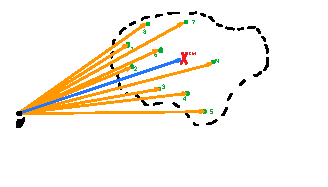
\includegraphics[width=6.5cm]{cm.pdf}
            \caption{Un sistema arbitrário con su respectivo centro de masa}
            \label{fig: centrodemasa}
        \end{figure}
    \end{marginfigure}

    \begin{definition}[\textbf{Centro de masa}]
        Corresponde a un punto del espacio en que se encuentra el sistema de partículas (discreto o continuo) en el cual es posible colapsar toda la masa del sistema, de modo que una fuerza arbitrária que interactue con alguna partícula del sistema se podrá transportar a dicho punto para conocer la mecánica del sistema (\Figref{fig: centrodemasa}). El centro de masa se define a partir de un promedio ponderado de toda la masa del sistema visto a continuación:

        \begin{align}
            \vec{r}_{CM} = \frac{1}{M} \sum_{\alpha =1}^{N} m_{\alpha} \vec{r}_{\alpha} \; \; \rightarrow  & \; \; \vec{r}_{CM} = \frac{1}{M} \int_{M} \vec{r} dm \\ 
            M = \sum_{\alpha = 1}^{N} m_{\alpha} \; \; \rightarrow  & \; \; M =  \int_{M}  \rho dV
        \end{align}
        
    \end{definition}

    \begin{definition}[\textbf{Momentum Lineal del Sistema}]
        gggg
    \end{definition}

    \begin{theorem}[\textbf{Teorema de Ejes paralelos}]
        \begin{equation}
            I_{{q}'}= I_{q}^{cm} + Md^{2}
        \end{equation}

        La demostración de este teorema tal y como se encuentra escrito aquí se le dejará al lector y se recomienda verlo como una simplificación del teorema de ejes paralelos real que se desarrollará más adelante.
    \end{theorem}
\end{document}